\chapter{Distributed Sensor Networks for Real-Time Air Quality Assessment}\label{ch:air-network}

As outlined in Chapter~\ref{ch:intro}, air quality is a critical factor
affecting human health and well-being. Many pollutants such as Ozone, \ce{CO},
\ce{NO2}, \ce{SO2}, and volatile organic compounds contribute to poor air
quality. Among the variety of sources, particulate matter (PM) plays a
significant role and has
been linked to increased mortality by numerous studies
\cite{pm-mortality-six-cities, pm-mortality-2}. PM is particularly interesting
because its deleterious impacts on human health derive from both from its
composition \textit{and} its ability to penetrate into the tissues of the human
body. Beyond the obvious impact on lung health, PM pollution has been linked to
cardiovascular mortality \cite{pm-cardiovascular}, increased chronic kidney
disease \cite{pm-kidneys}, and recently, increased incidences of
neurodegenerative diseases like Alzheimer's \cite{pm-neurodegenerative,
  pm-neurodegenerative-2}. Therefore, the accurate assessment of PM exposure is
of paramount importance.

Considerable research efforts have focused on the development of accurate
measurement techniques for particulate matter. Unfortunately, most
reference-grade instruments remain prohibitively expensive, stunting our ability
to characterize spatial and temporal PM variations at scales relevant to dense
urban and suburban environments. Recently, a new class of low-cost PM sensors
based on optical particle counting has emerged. These sensors can be calibrated
against reference instruments using machine learning methods to improve
measurement accuracy and reduce inter-sensor variability
\cite{pm-calibration-lakitha}. Using these devices, our research group has
developed a family of low-cost monitors for real-time PM measurement. To date
over 100 monitors have been built and distributed across the Dallas Fort Worth
metroplex and other Texas cities.

In this chapter, we first describe physical measurement methods for PM. We then
describe the monitors developed by the MINTS research group which collect
real-time PM measurements for a broad distribution of particle sizes. Finally,
we describe a comprehensive data pipeline developed for this dissertation to
processes measurement data and provide live visualization dashboards. The
system is designed using a collection of containerized, open-source tools to
guarantee reproducibility while ensuring the network can scale from hundreds to
thousands of sensors as it continues to expand. Later in Chapter~\ref{ch:havok},
we will analyze measurements collected by sensors in this network to develop a
physics-based method for outlier detection and forecasting of PM time series.

\section{Measurement of Particulate Matter}

Broadly speaking, instruments for measuring PM concentrations fall into one of
three categories:
\begin{itemize}
  \item \textbf{Federal Reference Methods} (FRM): These are methods which the US
    Environmental Protection Agency designate as the standard for PM measurement
    and may be used for assessing compliance with air quality regulations. The
    FRM for PM is \textit{gravimetric analysis} whereby particulate matter
    samples are collected onto a polytetrafluoroethylene (PTFE) filters which are
    then carefully weighed to determine PM concentration by combining the sample
    mass with a predetermined flow rate \cite{pm-federal-reference-method}. Standard
    measurements are for PM 2.5 and PM 10 which correspond to particles with an
    aerodynamic diameter of $\leq 2.5$ $\mu m$ and $\leq 10$ $\mu m$, respectively.
  \item \textbf{Federal Equivalent Methods} (FEM): These measurement techniques
    include \textit{Beta Attenuation Monitors}  (BAM), \textit{Tapered Element
      Oscillating Ribbon} (TOEM) monitors, and \textit{Optical Particle
      Counters} (OPC) based on light scattering. FEM methods are also approved
    by the US EPA for ambient PM monitoring.
  \item \textbf{Low-cost Sensors}: These sensors are much less expensive than
    FRM and FEM systems but are not approved by the EPA for assessment of
    compliance with government regulations. Most low-cost sensors are based on
    a simplified OPC design.
\end{itemize}
The PM sensors used in the MINTS sensing network fall into the low-cost OPC category.

\subsection{Optical Particle Counters}

Particulates scatter light according to their size and relevant physical
properties as described by Mie Scattering Theory for spherical dielectrics of
any radius. Optical particle
counters use light scattered off of particulates to estimate their size and
concentration. This method assumes particles are spherical and uses a
sufficiently slow flow rate so that, statistically speaking, particles enter the
sensing element individually. An example design for an OPC is shown below in
Figure~\ref{fig:opc-diagram}.

\begin{figure}[h]
  \centering
  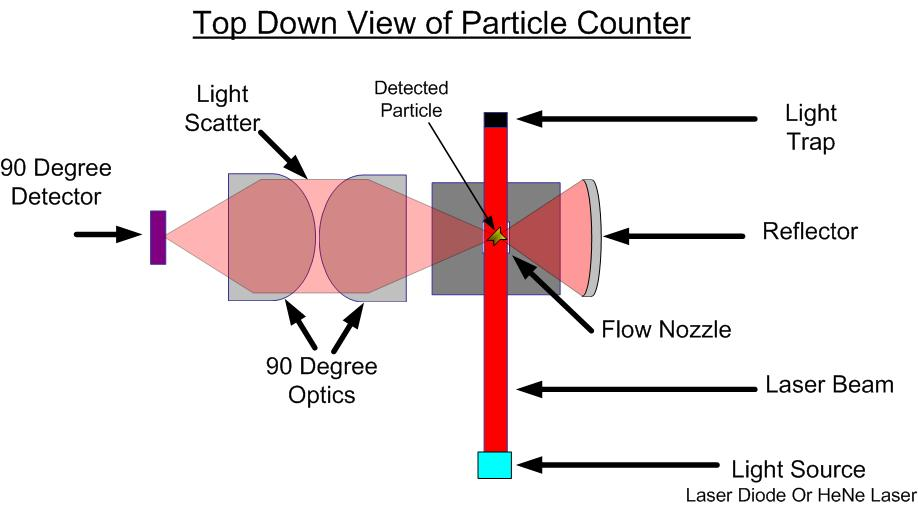
\includegraphics[width=0.7\columnwidth]{air-network/particle-counter.jpg}
  \caption{Optical particle counter: particulates are guided into the sensing
    element where a light source is then scattered off of the sample. This scattered
  light is then directed to detector. The inensity of scattered light is used to
distinguish particles by size. Image source: Morgan Polen, marked as public domain
(\url{https://en.wikipedia.org/wiki/File:Particlecounter.jpg}, accessed 2024-11-09). }
  \label{fig:opc-diagram}
\end{figure}

Particles are counted and sorted into distinct size bins based on the scattered
intensity with the detector oriented to limit the impact of index
of refraction on the scattered signal. For calibration,
most instruments use size-selected polystyrene spheres. Particle counts are then
converted into mass concentrations, for example PM 2.5 measured in $\mu g/m^3$.
This conversion is accomplished by assuming a constant particle density
consistent with observations for urban aerosols \cite{pm-density}.

An important consideration for OPCs is the impact of hygroscopic growth on
particle counts. When the humidity is sufficiently high, water tends to adsorb
onto particulates causing them to swell in size. Additionally, moistened
particulates may also agglomerate, coming together to form a larger particle
masses. This can significantly affect the accuracy of PM measurements by OPCs,
distorting in the estimated size distribution and causing overestimation
of the true particulate mass. For this reason, FEM instruments using the OPC method
often include humidity control and heating elements. This significantly improves
the accuracy of sensor measurements but decreases the sampling rate to $1-10$
minutes per reading while increasing power consumption and instrument cost.
With the growing interest in low-cost OPC-based sensors, a variety of
corrections using local temperature and humidity data have been developed
to account for this effect \cite{opc-corrections}.

The current iteration of air quality monitors designed by the MINTS research
group utilize the Pierra Systems IPS7100 Intelligent Particle Sensor. This
device is capable of measuring PM concentrations at 1 Hz across multiple size bins
to provide concentration measurements for PM $0.1$, $0.3$, $0.5$, $1$, $2.5$, $5$,
and $10$. Estimation of ultra-fine particulates is made possible due to the
detector's $1$ MHz sampling rate. We note that the $0.1$ $\mu m$ size bin, is
extrapolated from the measured size distribution. An example of an individual
IPS7100 sensor is shown in Figure~\ref{fig:ips7100}.

\begin{figure}[!h]
  \vspace{-1cm}
  \centering
  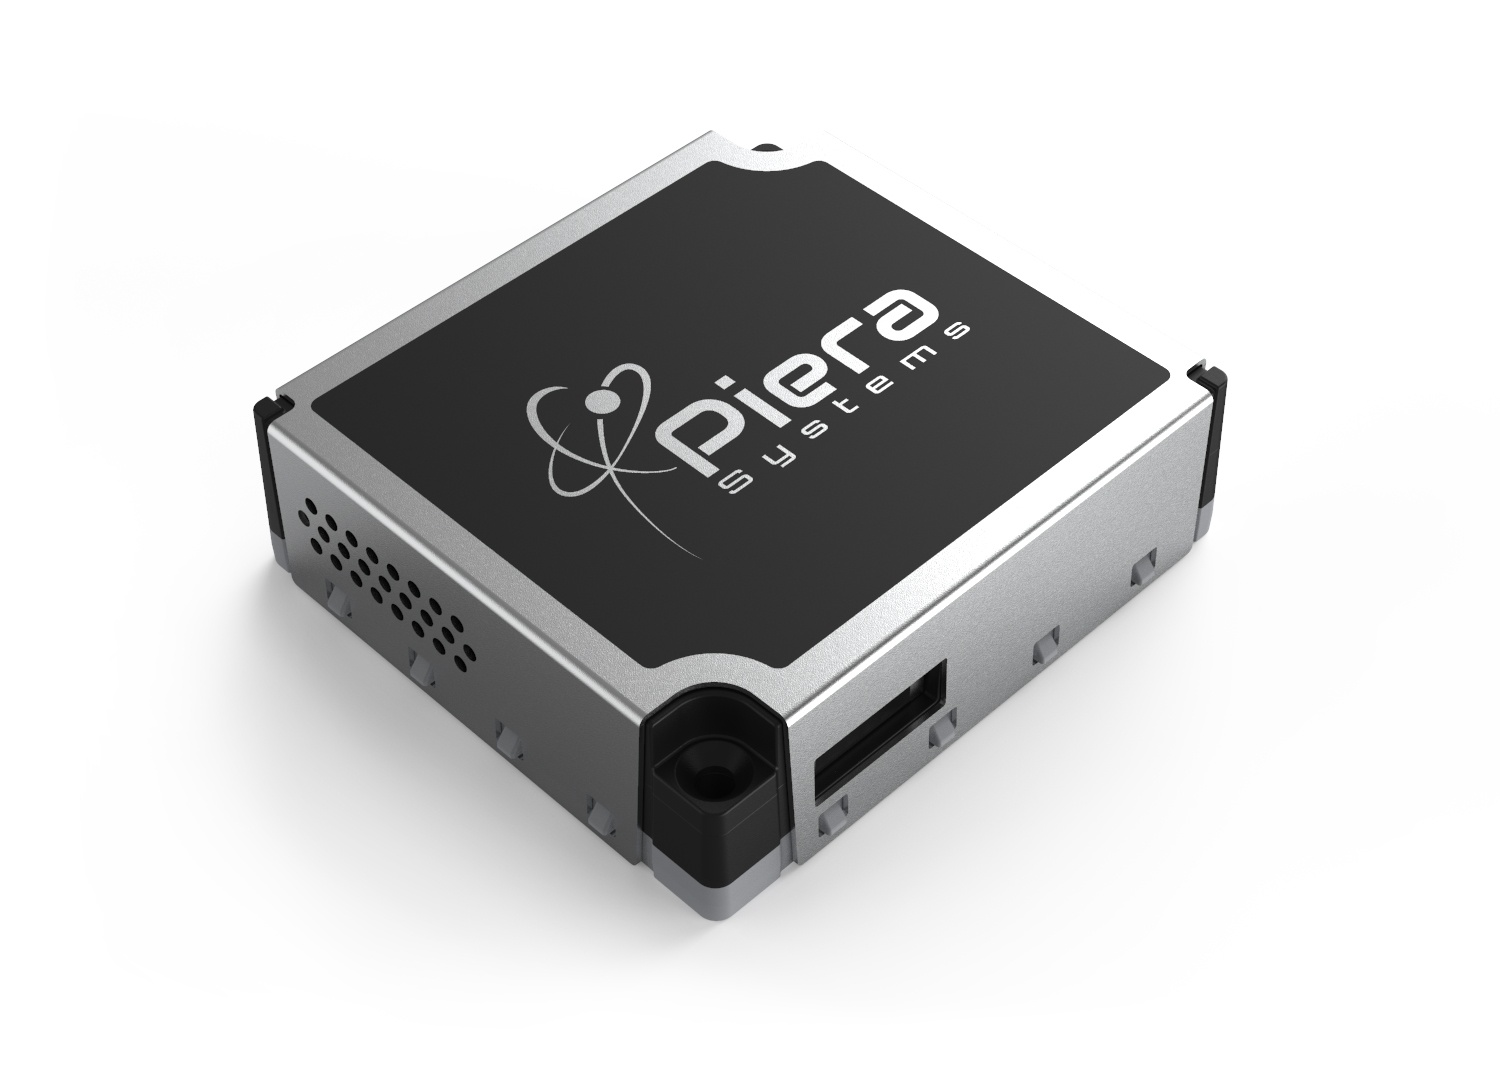
\includegraphics[width=0.4\columnwidth]{air-network/ips7100.jpg}
  \caption{The Pierra Systems IPS7100 Particulate Sensor.}
  \label{fig:ips7100}
\end{figure}

\section{A Low Cost Sensor Network For Air Quality Monitoring}


% The highly expensive cost to acquire, calibrate, and maintain reference grade
% air quality monitors makes it challenging to assess the importance of spatial
% and temporal variability on local air quality. Since factors such as weather,
% terrain, traffic, and the distribution of other sources can all effect local air
% quality, the development of low-cost sensing solutions is vital to address risks
% of poor air quality on local communities. To address this gap, we have developed
% a hierarchy of low-cost air quality monitors which we have deployed throughout
% the Dallas Fort-Worth (DFW) metroplex. In this section, we describe the relevant
% sensor types as well as a robust data processing and visualization pipeline
% developed to enable open access to high quality data.

\subsection{Sensor Nodes}

The sensor network is comprised of a combination of two types of nodes:
\textit{Central Nodes} and \textit{LoRa Nodes}. The Central Nodes are designed
to be deployed in locations with where dedicated power is available. Each
contains a variety of sensors including the IPS7100 for PM as well sensors for
VOCs, \ce{CO2}, \ce{NO_X}, ionizing radiation, incident light intensity,
sound levels, and meteorological variables including temperature,
pressure, relative humidity, and dew point. The powered Central Nodes are
equipped with a cellular modem to facilitate data transfer from their deployment
site.


Each Central Node supports a collection of $\sim~$10 LoRa nodes (named for the
long rage wireless transmission protocol) which can be separated by distances up
to $\sim$5 km or more if line of sight is established. These smaller sensors are self
powered using a combination of battery and solar cells, and each measures a
similar assortment of air quality parameters including particulate matter
concentrations, gas concentrations, and meteorological variables. Designs for
the two node types are illustrated in Figure~\ref{fig:mints-nodes}.

\begin{figure}[!hbt]
  \begin{subfigure}{.5\textwidth}
    \centering
    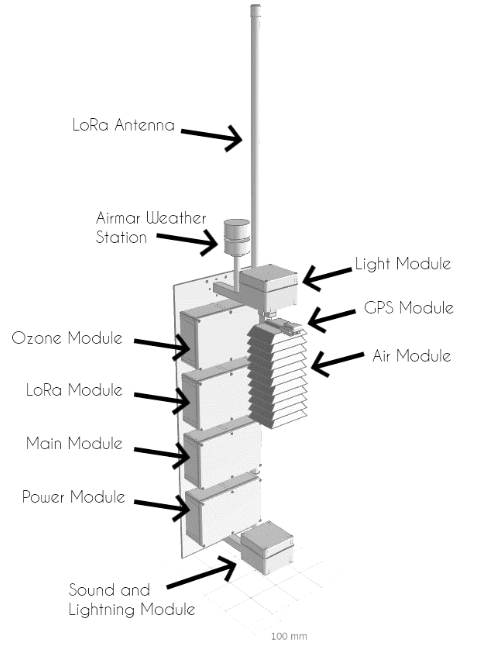
\includegraphics[width=.8\linewidth]{air-network/central-node.png}
    \caption{A 3d model of a Central Node}
  \end{subfigure}
  \begin{subfigure}{.5\textwidth}
    \centering
    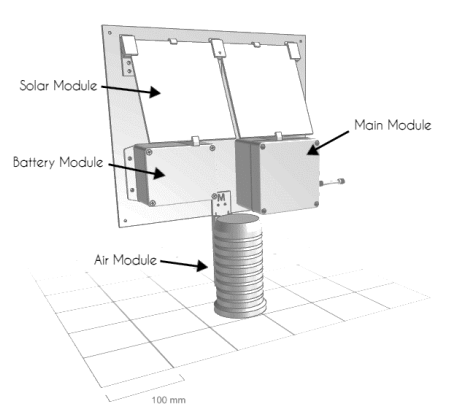
\includegraphics[width=.8\linewidth]{air-network/lora-node.png}
    \caption{A 3d model of a LoRa Node}
  \end{subfigure}
  \caption{Two types of nodes from the MINTS Air Quality network. Reproduced
    with permission from \cite{lakitha-thesis}}
  \label{fig:mints-nodes}
\end{figure}

Using the LoRaWAN protocol, Central and LoRa nodes form a low-power, wide-area
network through which data packets containing live measurements from each
LoRa node are transmitted to the nearest Central Node. The Central Nodes then
pass measurement data to a to a data processing backend using an MQTT
publish-subscribe model with their built-in cellular connection \cite{mqtt}.
Beginning in 2020, the first generation of nodes were assembled and installed as
shown in Figure~\ref{fig:sharedair-site}. In addition to sensors from MINTS, this
map also includes EPA reference sensors and sensors from the PurpleAir network.
\begin{figure}[!hbt]
  \centering
  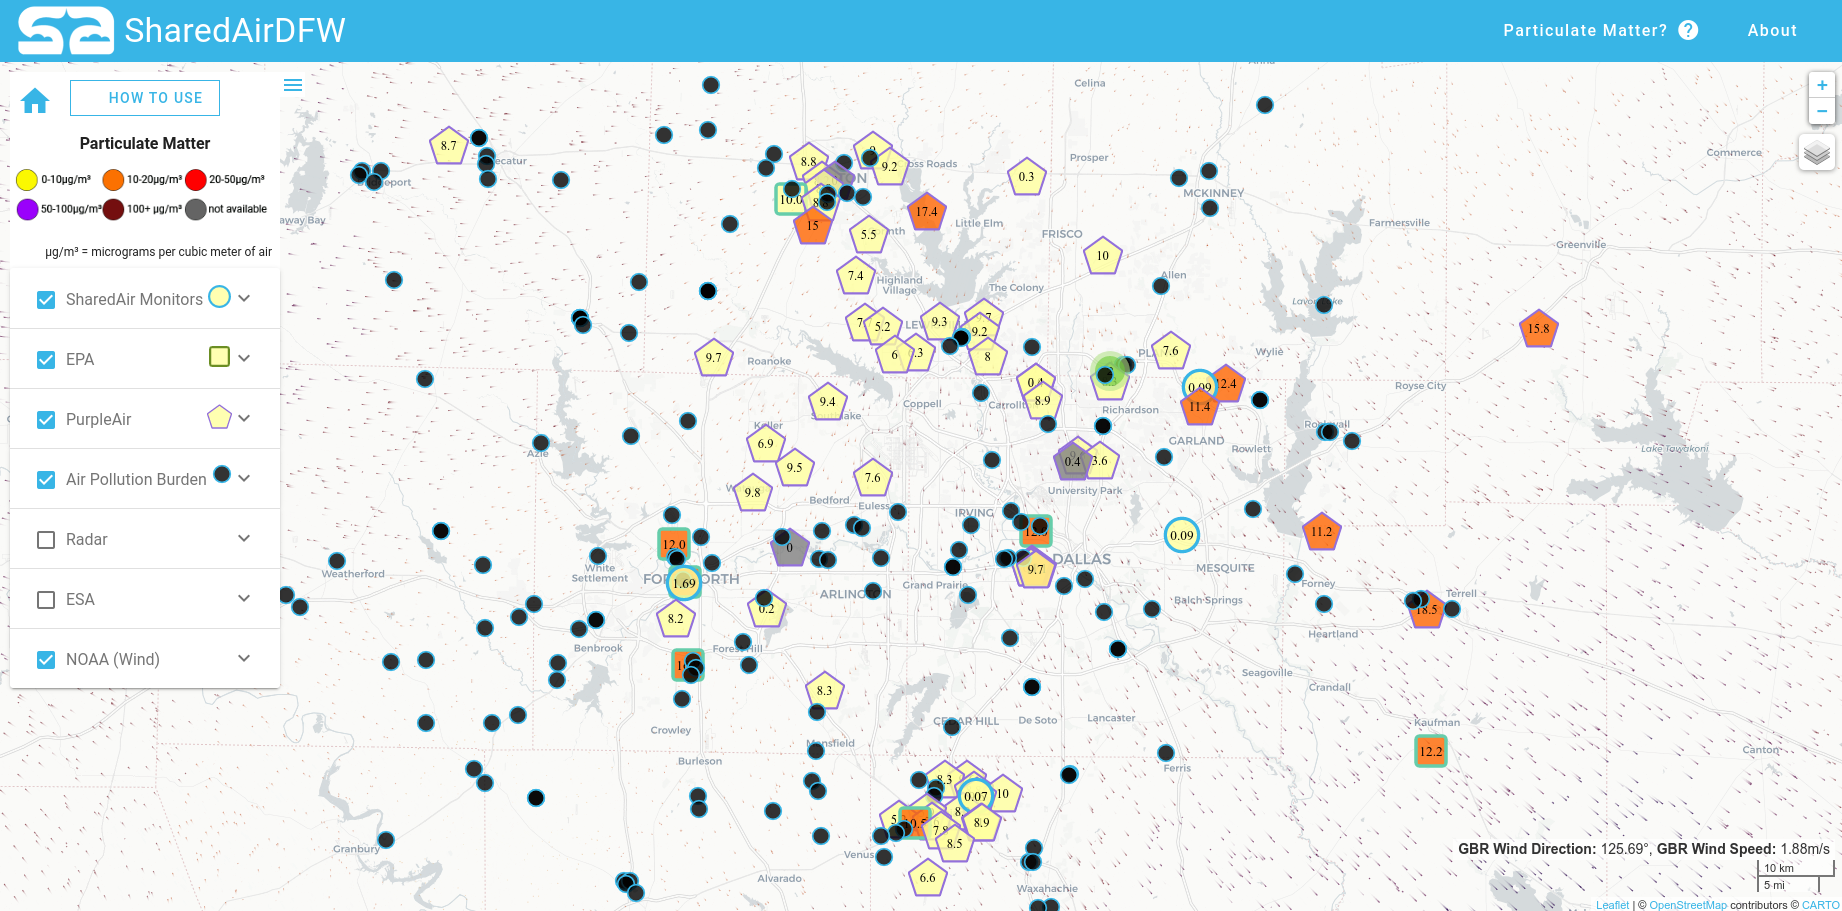
\includegraphics[width=0.85\columnwidth]{air-network/sharedairdfw-homepage.png}
  \caption{Interactive website displaying live sensor data on map. MINTS sensors
  are denoted with circular markers and additional data sources from EPA
  monitoring sites and PurpleAir monitors are included. Wind fields visualized
  using forecasts provided by NOAA.}
  \label{fig:sharedair-site}
\end{figure}


\subsection{The Data Pipeline}

To make real-time data available for public consumption and further analyses, a
containerized pipeline was implemented which combines a variety of open-source
data processing and visualization tools. \textit{Containerization} is a
method of encapsulating software together with
all of its dependencies, libraries, and configuration settings. Critically,
containerization makes software components such as databases and web servers
highly portable so that tools can be developed locally and then deployed to
remote systems.

Containers are defined using \textit{Dockerfiles} and can be networked together
with common data storage to achieve complex workflows. The pipeline developed
for the MINTS air quality network combines three containerized open-source tools:
\begin{itemize}
\item \textbf{NodeRed}: Developed by IBM, this tool allows the creation of
  custom data processing workflows by defining directed acyclic graphs (DAGs)
  corresponding to individual processing tasks. This tool is utilized to subscribe to
  each sensor's MQTT topics and decode binary data packets into individual
  sensor measurements. Processed data are then injected by NodeRed into a
  time series database. A key advantage of NodeRed is the vast set of
  pre-implemented processing nodes which provide an easily maintainable, low-code
  environment. Workflows are saved as JSON files which can be version controlled
  for replicability.
\item \textbf{InfluxDB}: An open source time series database optimized
  for large cardinality datasets. By storing processed data in InfluxDB, we are
  able to provide queryable access to live and historic measurements.
\item \textbf{Grafana}: A visualization platform for creating live, interactive
  dashboards. Grafana is connected to InfluxDB to provide detailed, real-time
  displays for each sensor in the network. These dashboards visualize data from
  \textit{all} incoming measurements from each node.
\end{itemize}

\begin{figure}[!h]
  \centering
  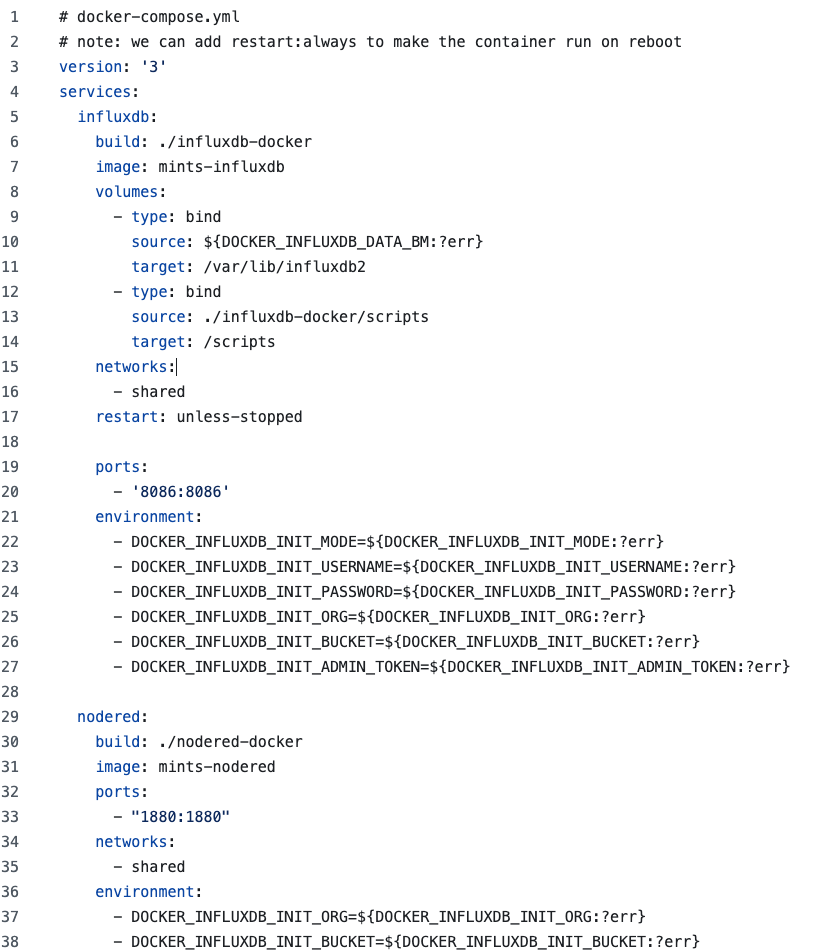
\includegraphics[width=0.95\columnwidth]{air-network/compose-snippet.png}
  \caption{Snippet of the \texttt{docker-compose.yml} file showing the
    combination of InfluxDB and NodeRed. Each individual container can define
    network ports, shared data volumes, and environment variables.}
  \label{fig:compose}
\end{figure}

Container orchestration is accomplished using YAML files like the examples shown
in Figure~\ref{fig:compose}. For local development, the \texttt{docker-compose}
tool can be used \cite{docker-compose}. However, this requires root permissions
which is unreasonable for remote servers. The \texttt{podman-compose} tool can
be used in these scenarios to achieve the same effect \cite{podman-compose}.
Conveniently, \texttt{podman} accepts the dame \texttt{Dockerfile} and
\texttt{docker-compose.yml} files. The data processing pipeline is currently
deployed on a remote virtual machine managed by the University of Texas at
Dallas. Migration of the pipeline to the cloud via Amazon Web Services is
currently in progress.

Figure~\ref{fig:influxdb} shows an example view of the InfluxDB time series
database web interface (\url{http://mdash.circ.utdallas.edu:8086}, last accessed
2024-09-12). Each node in the network is assigned a unique device name which is
used to identify the time series measurements for each sensor in the node.

\begin{figure}[!h]
  \centering
  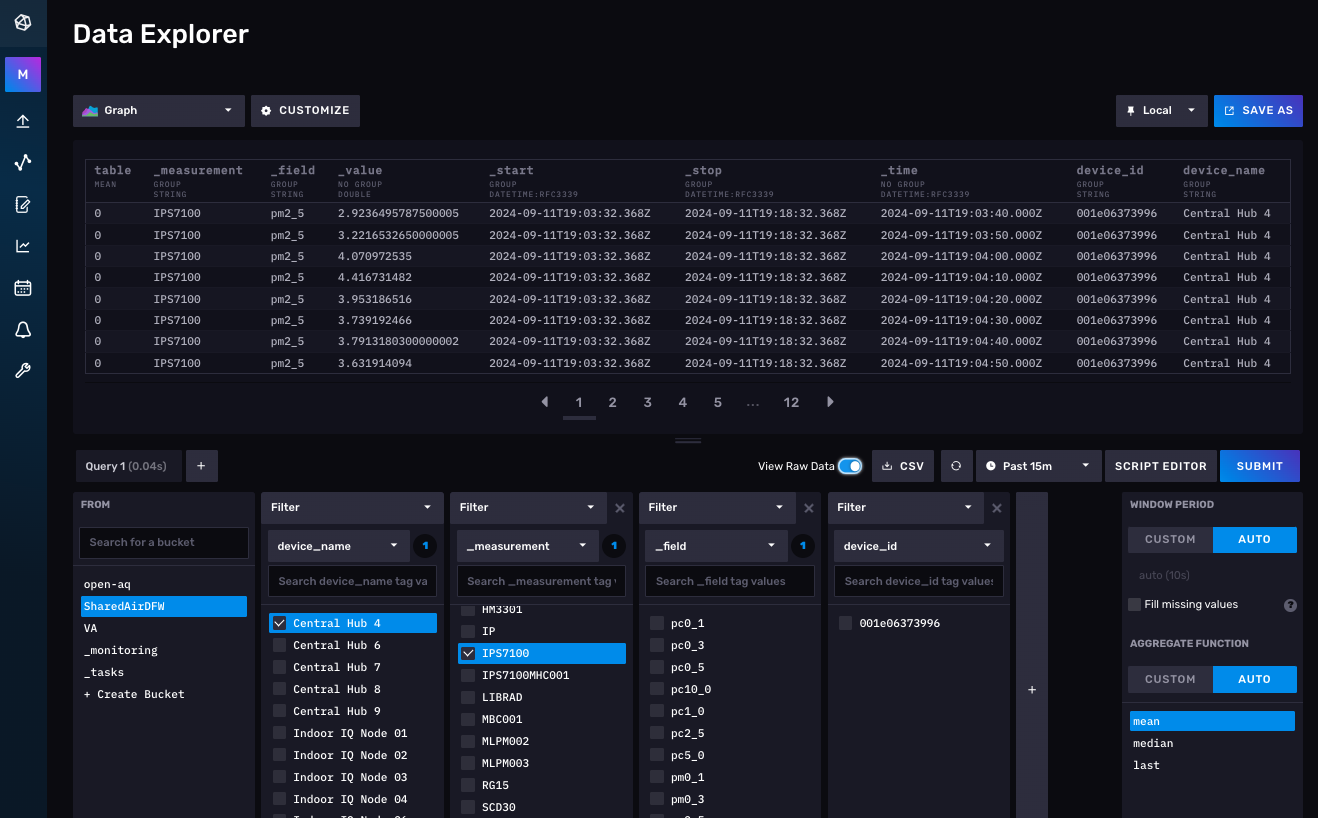
\includegraphics[width=0.9\columnwidth]{air-network/influxdb.png}
  \caption{A view of the time series data accessible from the InfluxDB database.
  Each sensor is assigned a unique device name. Time series for individual
  sensor measurements can be identified by the sensor name and the specific
  measurement.}
  \label{fig:influxdb}
\end{figure}

Interactive dashboards for each node in the network are deployed using Grafana
(\url{http://mdash.circ.utdallas.edu:3000}, last accessed 2024-09-12). An example
dashboard for a central node is shown below in Figure~\ref{fig:grafana}. Every 5
seconds, Grafana queries InfluxDB to update each graph with the latest values.
These real-time data feeds provide invaluable insight into the local air
quality. Including relevant meteorological parameters together with PM
measurements provides critical context when interpreting PM data. Additionally,
automated alerts triggered by live measurements can be set to provide early warnings
for high pollution episodes or sensor degredation.

\begin{figure}[!h]
  \centering
  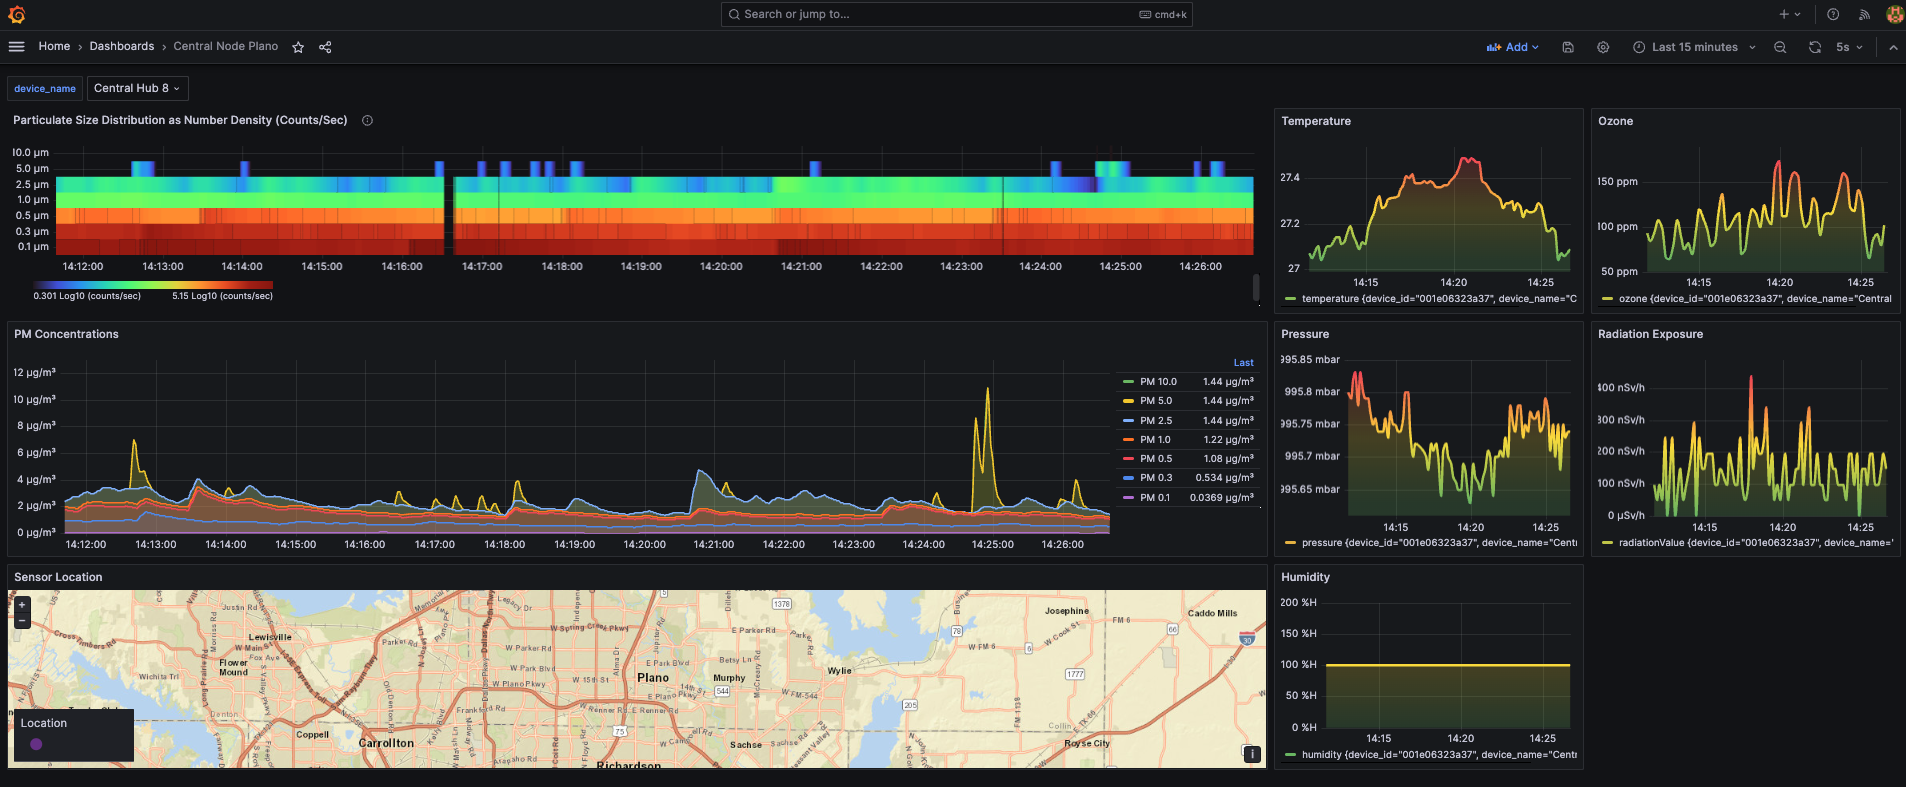
\includegraphics[width=0.95\columnwidth]{air-network/grafana.png}
  \caption{Example grafana dashboard for a central node. Live graphs showing the
  distribution of particle sizes together with mass concentrations for each PM
  size fraction are visualized together with meteorological data for
  temperature, pressure, and humidity.}
  \label{fig:grafana}
\end{figure}
All configuration files required to fully reproduce the data pipeline are
version controlled using git and hosted remotely on github \cite{mints-docker}.

To provide additional redundancy and easy access to large batches of historical
time series, all network data is synchronized daily to a remote file store on
the \textit{Open Storage Network} (OSN). OSN is a petabyte scale, NSF funded,
distributed data storage system which provides open access and long-term storage
for scientific datasets \cite{osn}.


